\section{Implementation}
In this section we will go through the implementation of the applications which use the camera from the device and the OpenCV library to for the positioning algorithm 

\subsection{Architecture}

Figure \ref{fig:device-setup} shows the arrangement of the devices on the table. It shows a device on a stand with its camera facing down onto the table which does all the vision calculations. There are a multiple of devices on the table which come together to become an ad-hoc ubiquitous surface. From now on the device on the stand will be called CameraApp and the devices on the table will be called TableApp.
\begin{figure}[H]
\centering
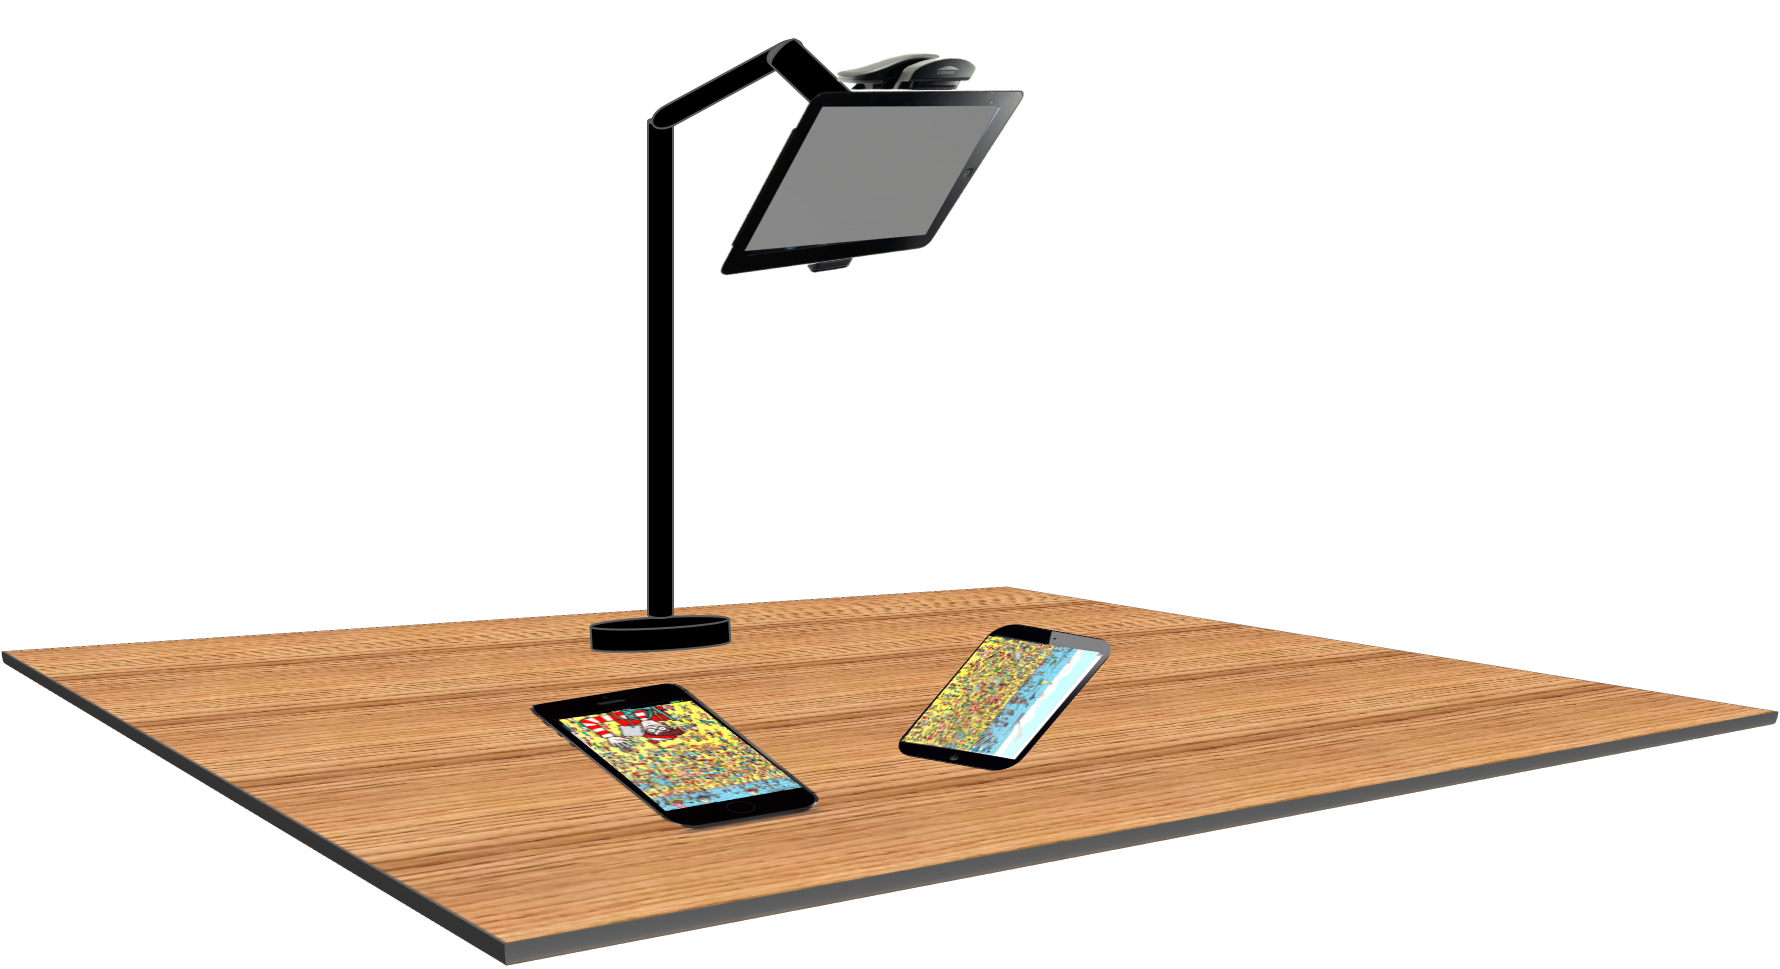
\includegraphics[width=\textwidth]{device-setup}
\caption{The setup of HuddleTable using the camera of a Mobile device}
\label{fig:device-setup}
\end{figure}


Vision calculations, done by CameraApp, locates the coordinates of all the TableApps and store them to the Firebase data store. As soon as the position gets updated the TableApp gets a notification with its location on the table and show the part of the canvas at that location.

\subsection{Database Design}

Firebase saves the information in a JSON format on its database as a (key, value) pair. Figure \ref{firebase_design} shows the design we went with for our project. We decided to proceed with a tree like structure and delegating some control to the users of their different sessions. The database is designed in a way that the users can get all the information they need depending on their session name. 

The picture is colour coded, the yellow nodes are the ones that has multiple children. The green nodes are the ones that are dynamically named, Session Name is the name that the user inputs into the application at the beginning explained more in Section \nameref{cameraapp}. The background colour is the colour that the devices flash initially, this will be explained more in Section \nameref{tableapp}. The background colour is the identification technique we are using to detect the devices and query the database. 

The \emph{numOFDevices} is the number of Devices that are in this session on the table. \emph{Zoom} is the value that the canvas is zoomed to in the session, and position is the position of the device that is identified by that particular background colour.

\begin{figure}[H]
\centering
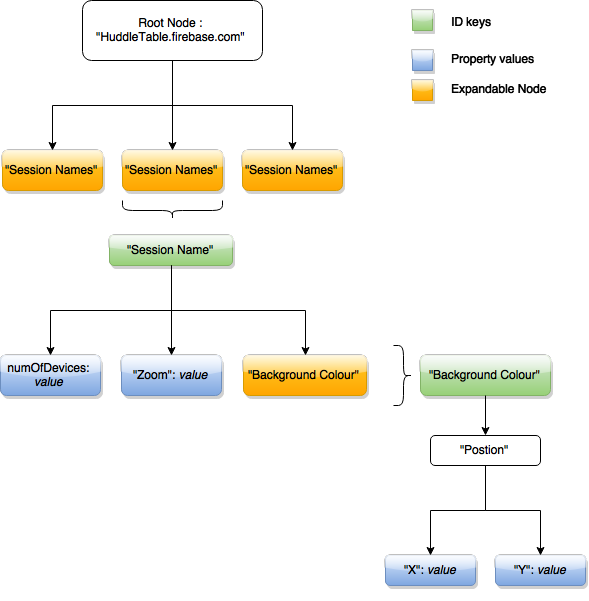
\includegraphics[scale=0.7]{firebase_design}
\caption{My Firebase database design}
\label{firebase_design}
\end{figure}

\subsection{Database API} 

We have created a simple, extendable API which would enable future developers of this application to harness the incredible power of Firebase. We have a class called \emph{Huddle}, which takes in a view that the data store is meant to manipulate and also the reference to firebase datastore. It is created using a singleton pattern so that only one instance of it could ever be created. We have a configure method which allows the developer to use bespoke firebase reference and also gives the Huddle Class the view that it can manipulate

\emph{private Huddle()}\\
A private constructor because it is a singleton patter

\emph{public static configure(Firebase ref, View v )}
This function will configure the Huddle Object to have the reference and the view needed for the class to function.

\emph{double getZoom()}\\
This is a function that be user by developers for their own bespoke application. We also use it for our automatic scrolling in the application. By having a Firebase \emph{ValueListener} set on zooom, every time the value gets changed an event gets fired which is caught by the listener.

\emph{getNumberOfDevices()}\\
Similar to the get zoom function, this is a method with a Firebase \emph{SingleValueListener} which only used once at the initialisation of the TableApp and the the listener automatically detaches.

\emph{getPosition()}\\
Similar to the getZoom() method, this has a  \emph{ValueListener} which is used to keep track of the internal state of the TableApp and update the view accordingly.

\emph{getAllPosition()}\\
This is a function that we have not used, however we have allowed the users to get the background colours and the location of all the devices in the ``Huddle" which the developers might use.

\emph{setZoom(double)}
This is a function we wrote so that the object could update the zoom of the view to the data store.

\emph{setPosition(Position)}
This is a function we wrote so that if the user decide to have accelerometer or some other external sensor readings that they want to use to get better positioning result they could update the position. This function currently is used by the CameraApp.

We have deliberately not giving the user control to update all the positions of all the devices i.e setAllPosition() as we believe this would be misused most probably.



\subsection{Applications}
For this concept to come to life we had to create two different applications. One of them is the replacement application for the camera and the laptop in the HuddleLamp project, called the \emph{CameraApp} and the other is the application for the devices on the table, called the \emph{TableApp}. This application should be able to deal with gesture control and interaction since we do not have depth sensors in this arrangement.

As you can see from our database design,the whole idea hinges on the ``session name", therefore both applications start off on a similar screen where the users can type in the session name. Figure \ref{session_screen} shows the session screen. 
\begin{figure}
\centering
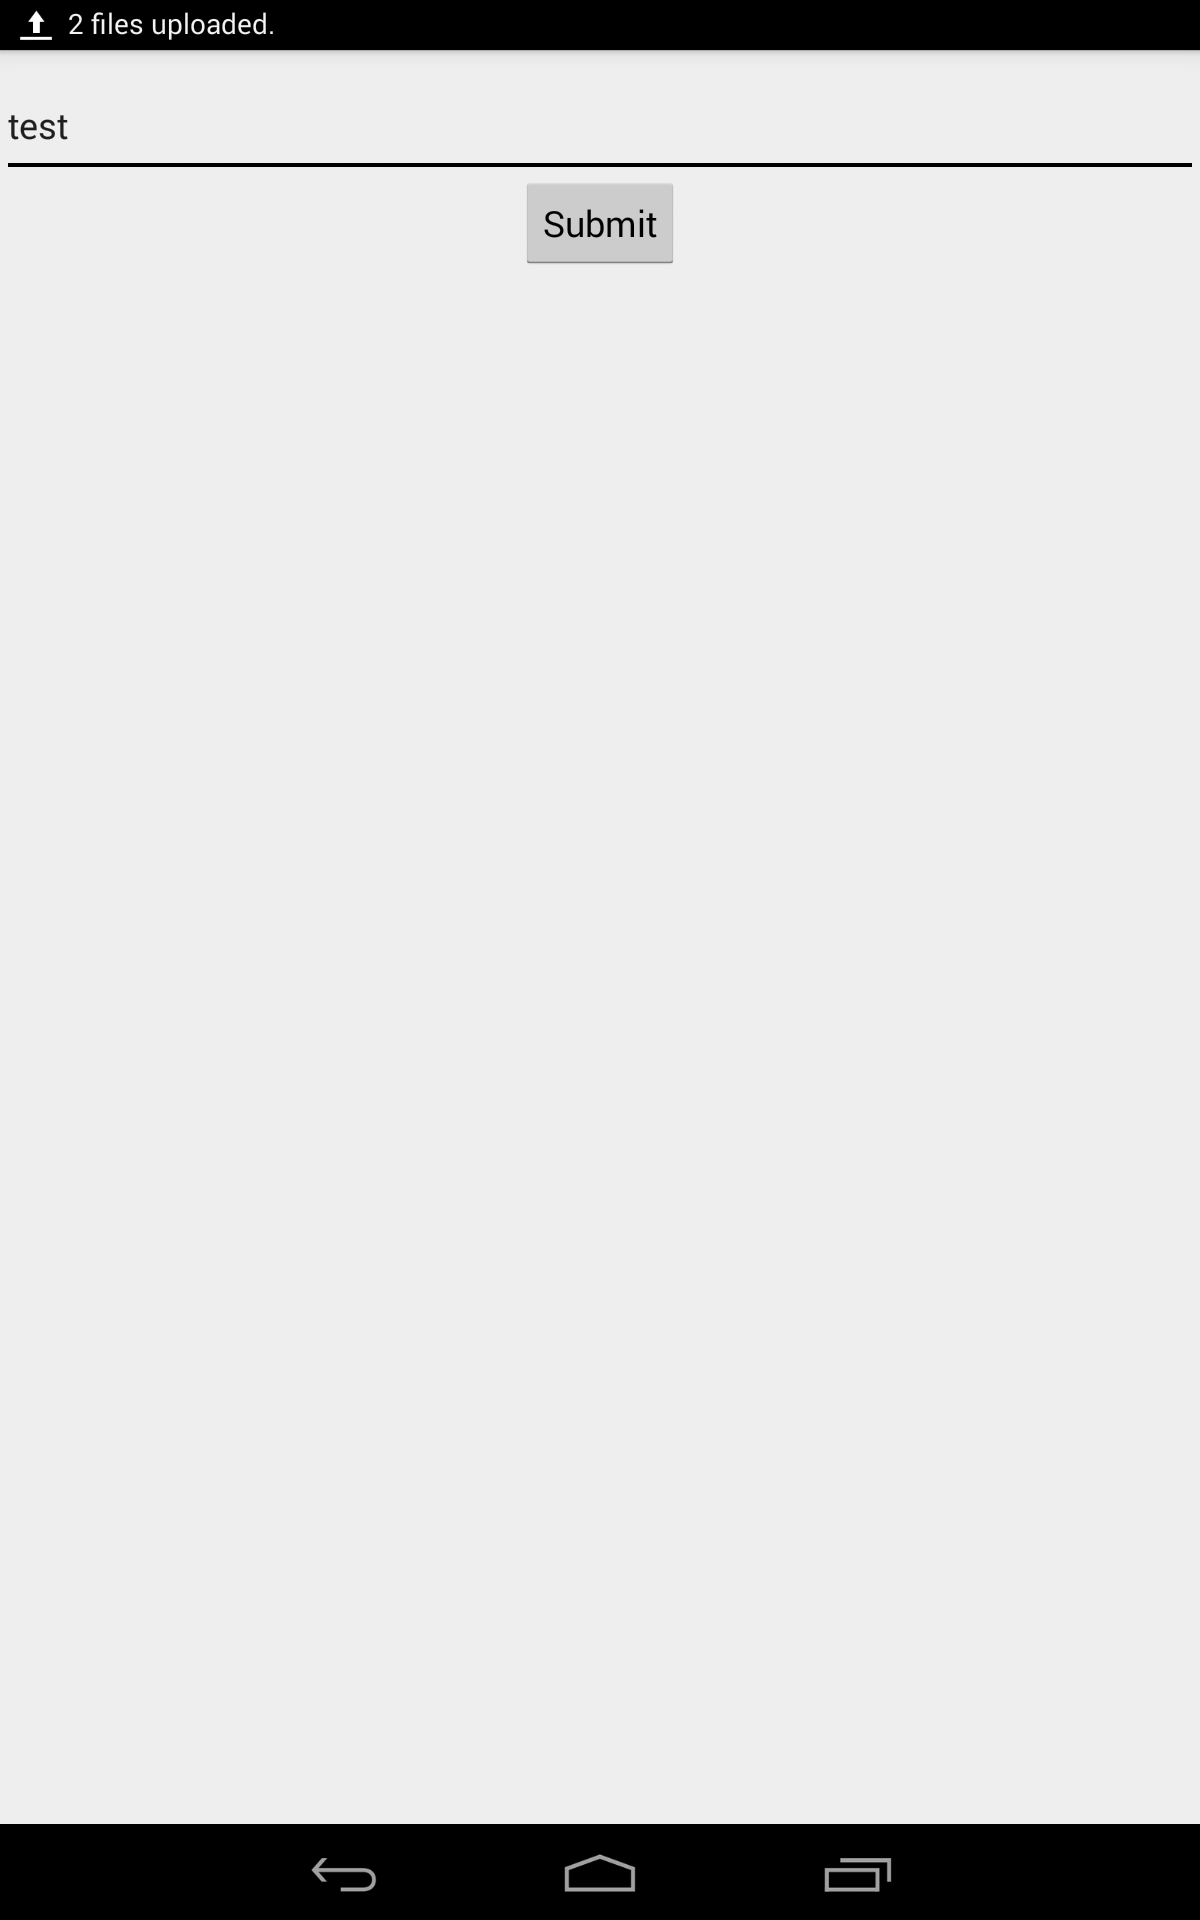
\includegraphics[scale=0.1]{session}
\caption{Shows the screen where the user input the name of the session}
\label{session_screen}
\end{figure}
\subsubsection{CameraApp} \label{cameraapp}

CameraApp is the main contribution in this Chapter. The primary aim of the CameraApp was to detect and identify devices on the table. Our research in Section \ref{device_identification} shows that the most efficient method for identification in this scenario would be colour detection. To simplify the problem and to reduce the chance of overlapping we have decided to limit the colours to just the primary colours. This would mean there would be a clear distinction between the colours, making it easier for the CameraApp to identify the position.
\begin{figure}[H]
    \centering
    \begin{subfigure}[b]{0.47\textwidth}
        \centering
        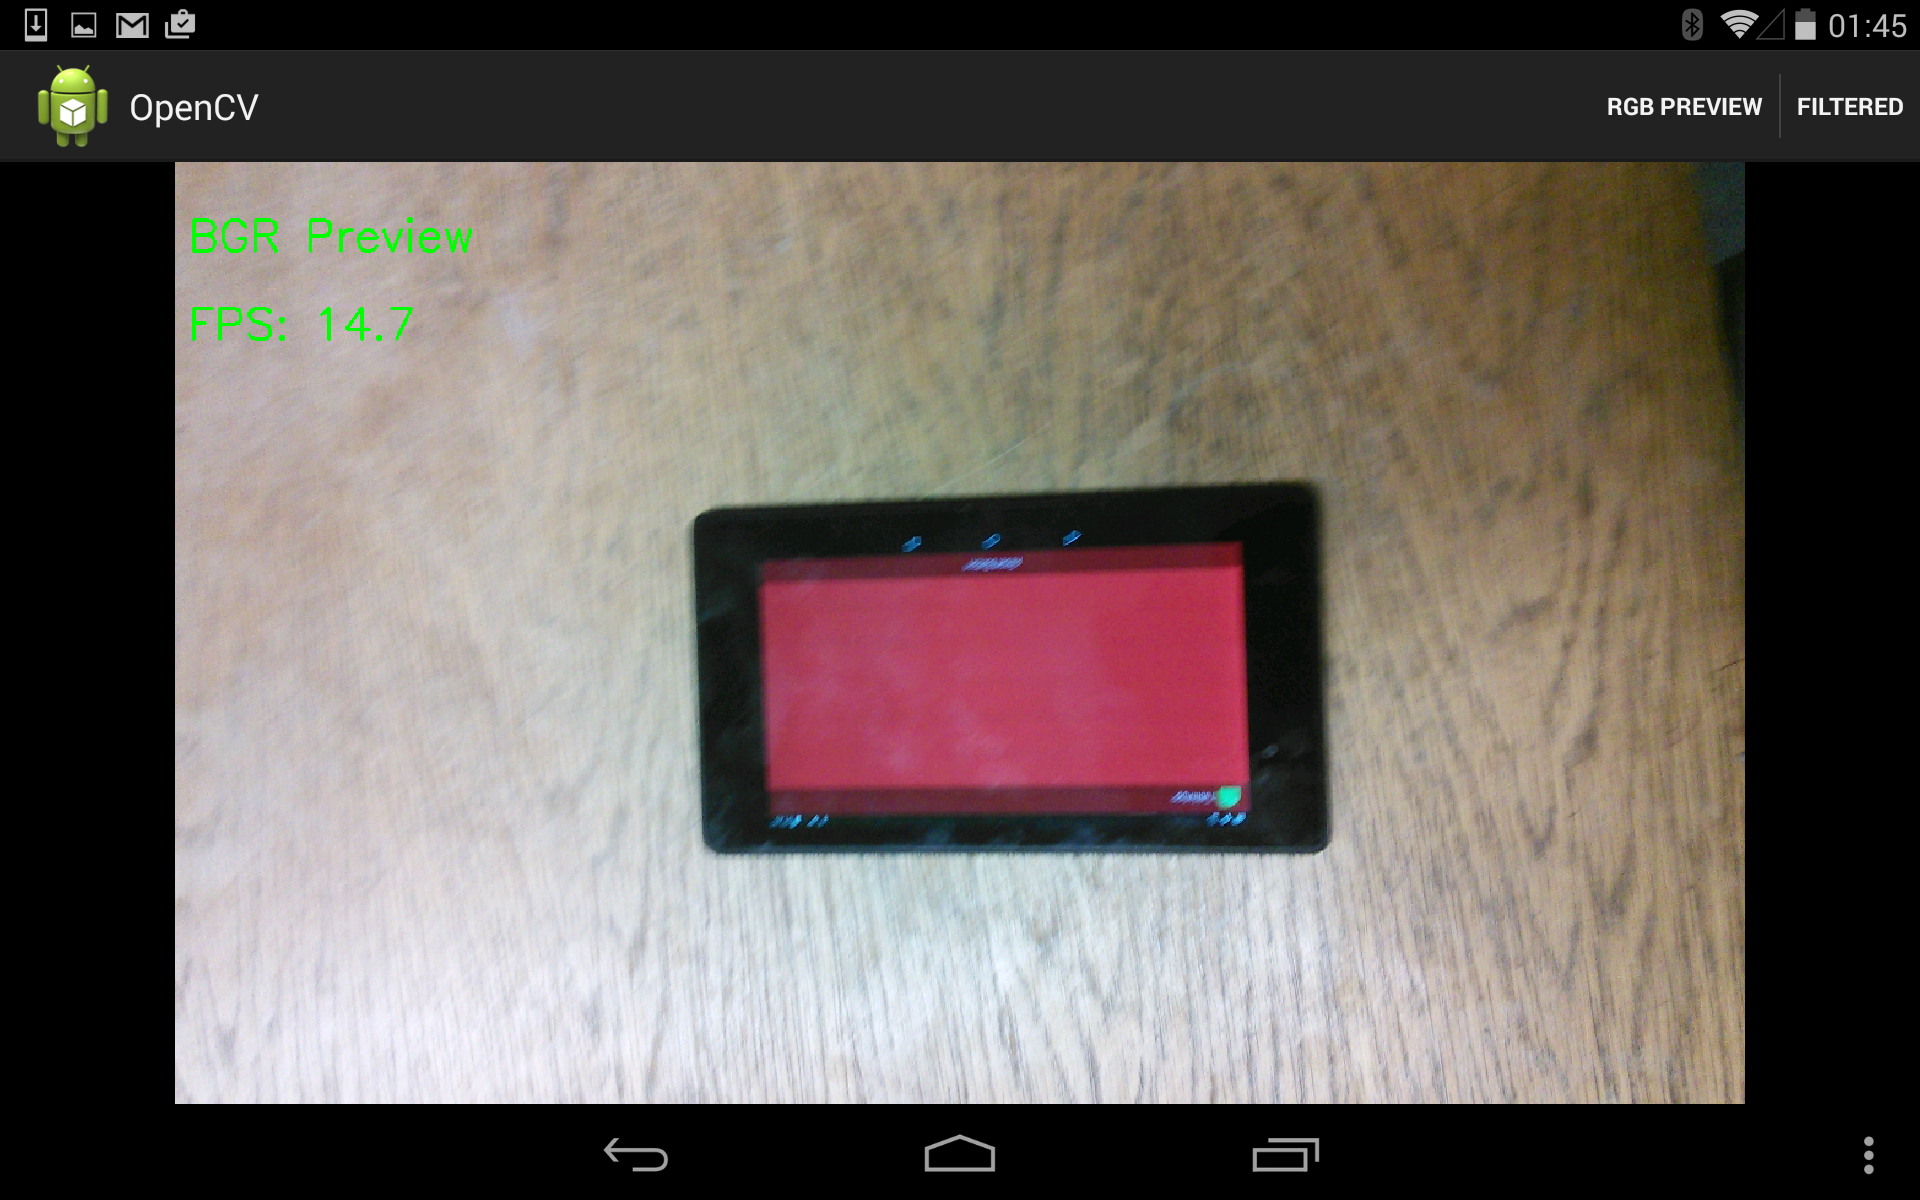
\includegraphics[width=\textwidth]{red(rgb)}
        \caption{A screen with Red area showing}
        \label{red_screen}
    \end{subfigure}
    \hfill
    \begin{subfigure}[b]{0.47\textwidth}
        \centering
        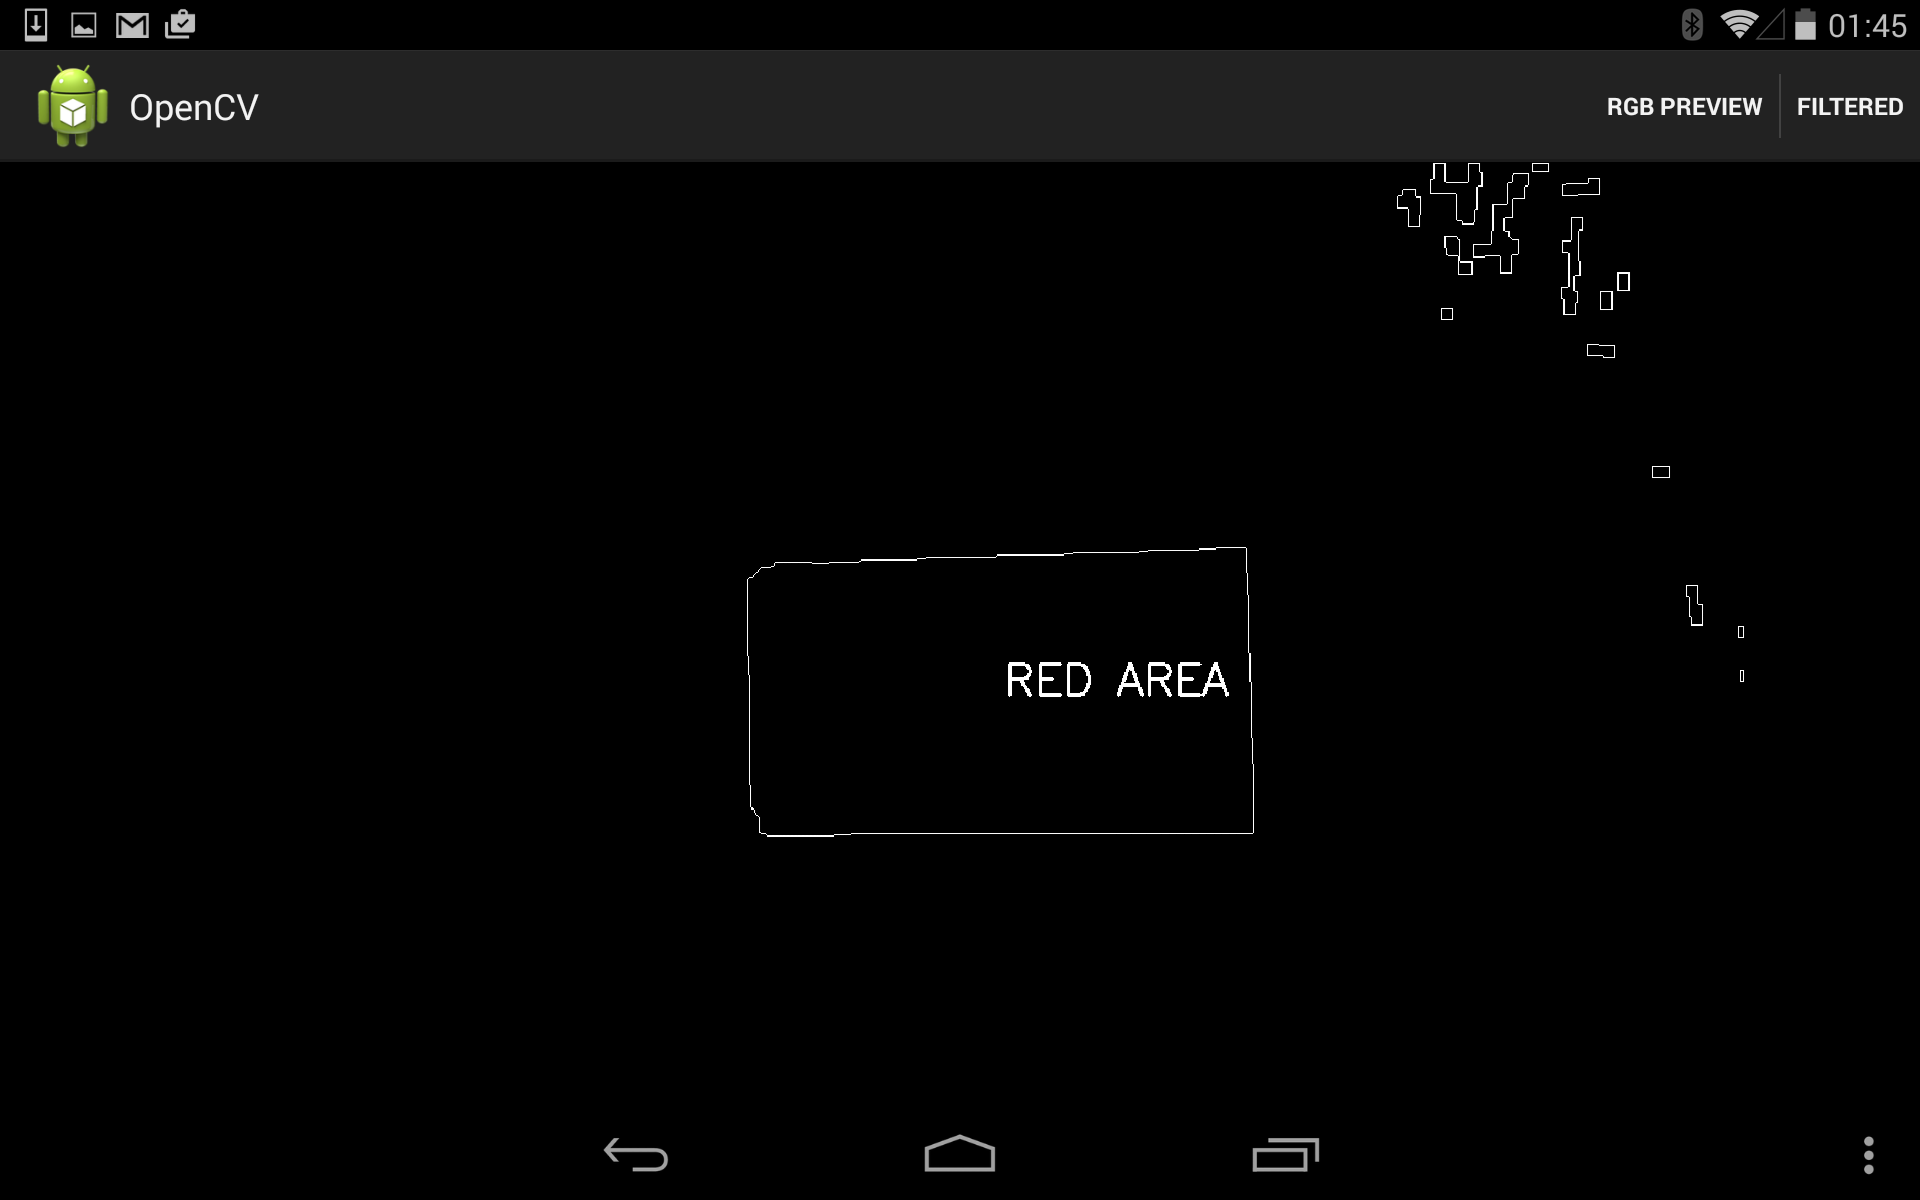
\includegraphics[width=\textwidth]{red(filtered)}
        \caption{Same frame filtered for Red}
    \end{subfigure}
    \hfill
    \caption{Screenshot of the application working for Red area}
     \label{filtered_red}
\end{figure}
As a proof of concept, and as an initial milestone we decided to try and get the CameraApp to detect large red surfaces. We had to determine the range for red colour in Hue, Saturation, Value (H, S, V) format and then filter the image for that range. Table \ref{colour_range} shows the various ranges for different colours. Figure \ref{filtered_red} shows the result of the application working for red colour.

\begin{table}[h]
\centering
\begin{tabular}{|c|c|}
\hline 
Colour & (H, S, V) Ranges\tabularnewline
\hline 
\hline 
Red & \begin{tabular}{@{}c@{}}(0, 100, 100) to (10, 255, 255) \\ \& \\ (160, 100, 100) to (179, 255, 255) \end{tabular} \tabularnewline
\hline 
Green & (40, 100, 100) to (75, 255, 255)\tabularnewline
\hline 
Blue & (100, 0, 0) to (120, 255, 255)\tabularnewline
\hline 
\end{tabular}
\caption{A table to show the Hue, Saturation and Value ranges used for the colours Red, Green and Blue}
\label{colour_range}
\end{table}

The next logical step was to get the position of the red object and store it in our data store in Firebase. This was made easier by using same key values for both applications such as, position, colour name etc. By using the same Enum of Colours for both apps we were able to ensure that the colour name saved onto Firebase would be identical and Figure \ref{id_string} shows the final strings which were then used as the key for other values such as position, number of devices and zoom.

\begin{figure}[H]
        \centering
            \begin{subfigure}[b]{0.47\textwidth}
        \centering
        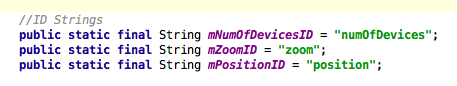
\includegraphics[width=\textwidth]{id_string}
        \caption{Strings used as the keys}
        \label{id_string}
         \end{subfigure}
    \hfill
    \begin{subfigure}[b]{0.47\textwidth}
        \centering
        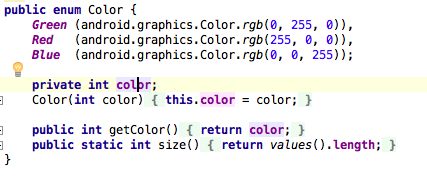
\includegraphics[width=\textwidth]{colour_enum}
        \caption{Colour Enum}
        \label{colour_enum}
    \end{subfigure}
    \hfill
\end{figure}

We used the view of the camera app for the coordinate system. By getting the position of the red object on the screen, and translating it using the function \emph{convertToPosition()} that we wrote, we worked out the position. We saved the data obtained as a position object onto our data store.

The next step in the evolution of the app was to filter for other colours, so that the camera could see and save these positions as well. Figure \ref{filtered_multiple} shows the scenario where the CameraApp was able to detect a red and green object in the same image and shows their respective positions. This milestone was achieved by making copies of each frame and then filtering the frames for different colour ranges. So in our case we had to make 4 copies (2 X red, blue and green) and filter them and then merge them using a weighted sum of all the arrays. OpenCV had a function called \emph{Core.addWeighted()} which was able to do this for us.
\begin{figure}[H]
    \centering
    \begin{subfigure}[b]{0.47\textwidth}
        \centering
        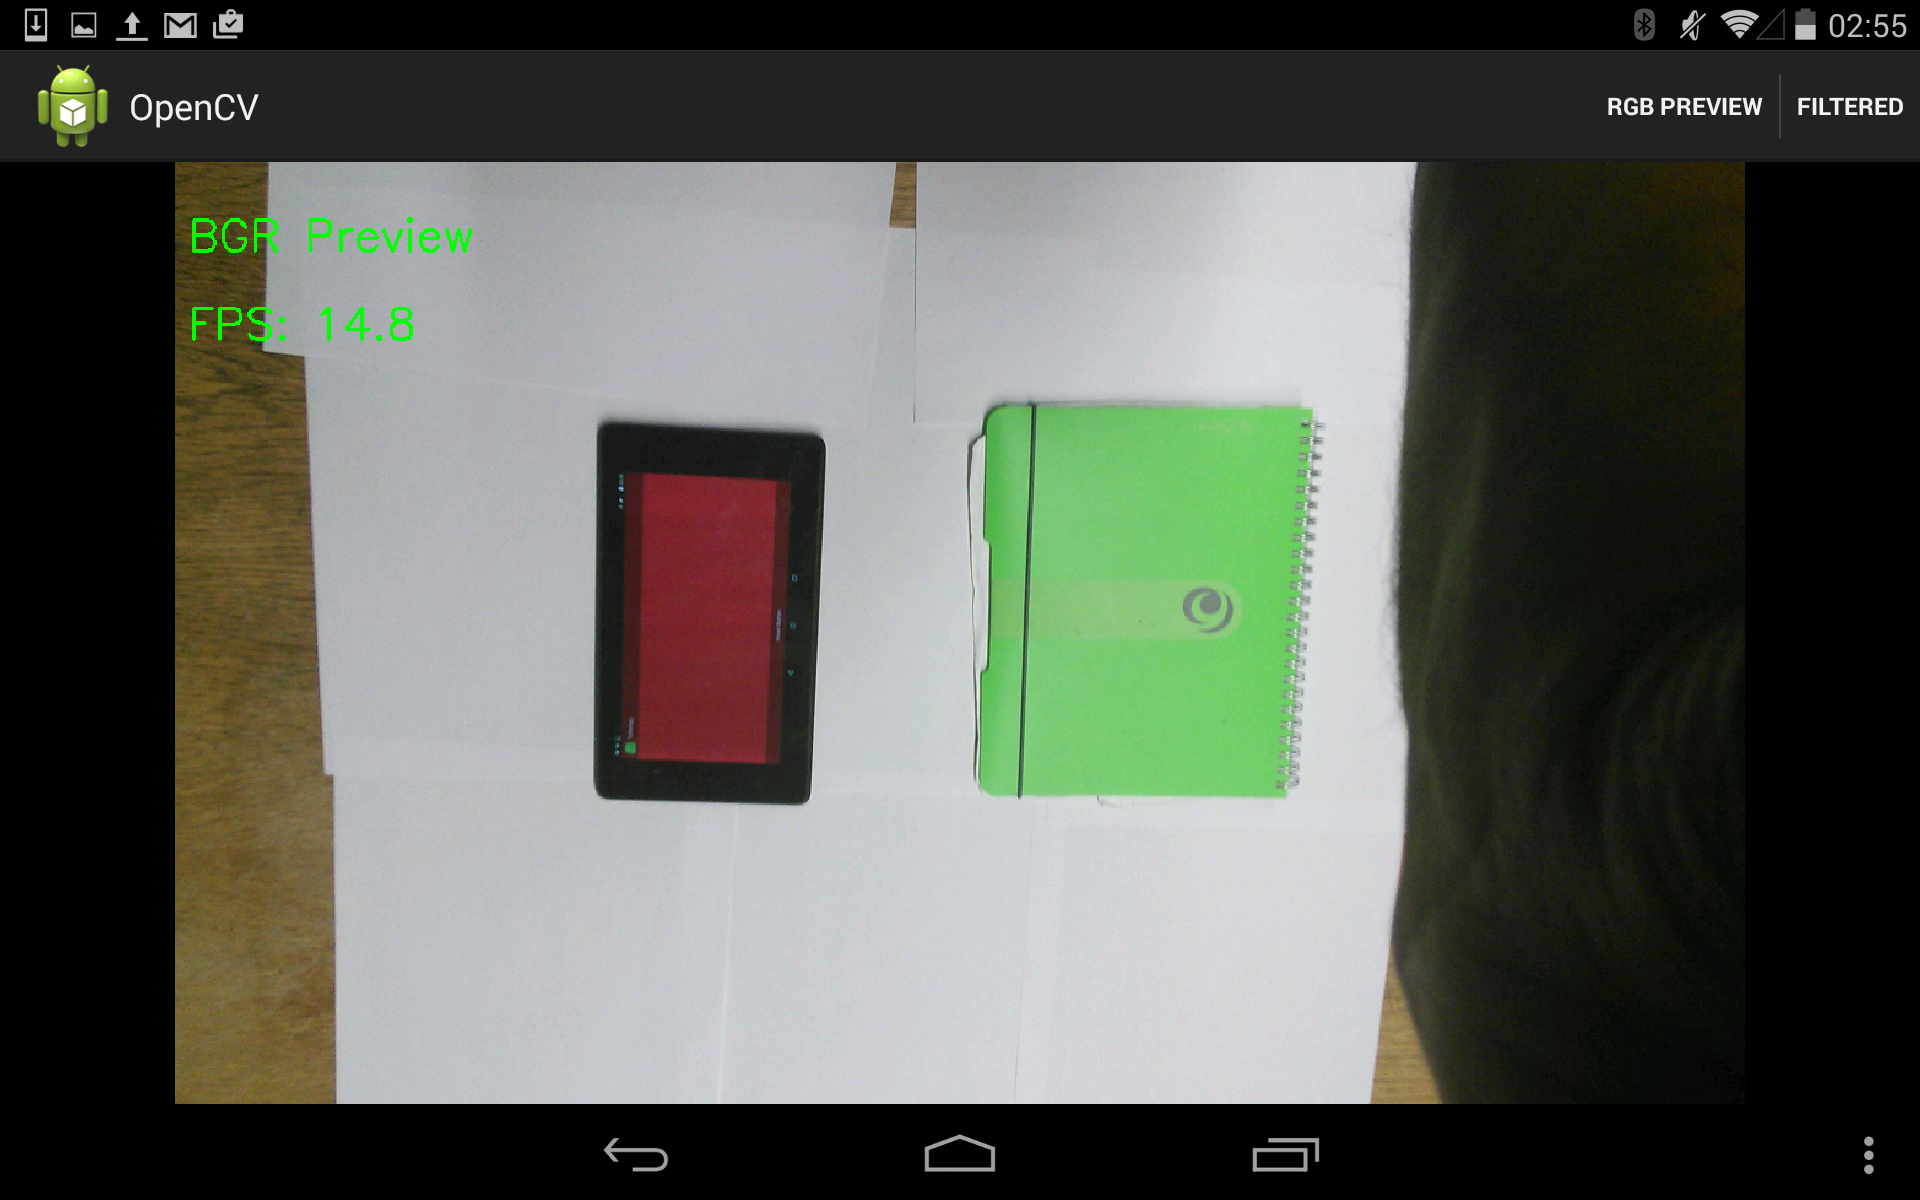
\includegraphics[width=\textwidth]{multiple(rgb)}
        \caption{A screen with Multiple colour area showing}
    \end{subfigure}
    \hfill
    \begin{subfigure}[b]{0.47\textwidth}
        \centering
        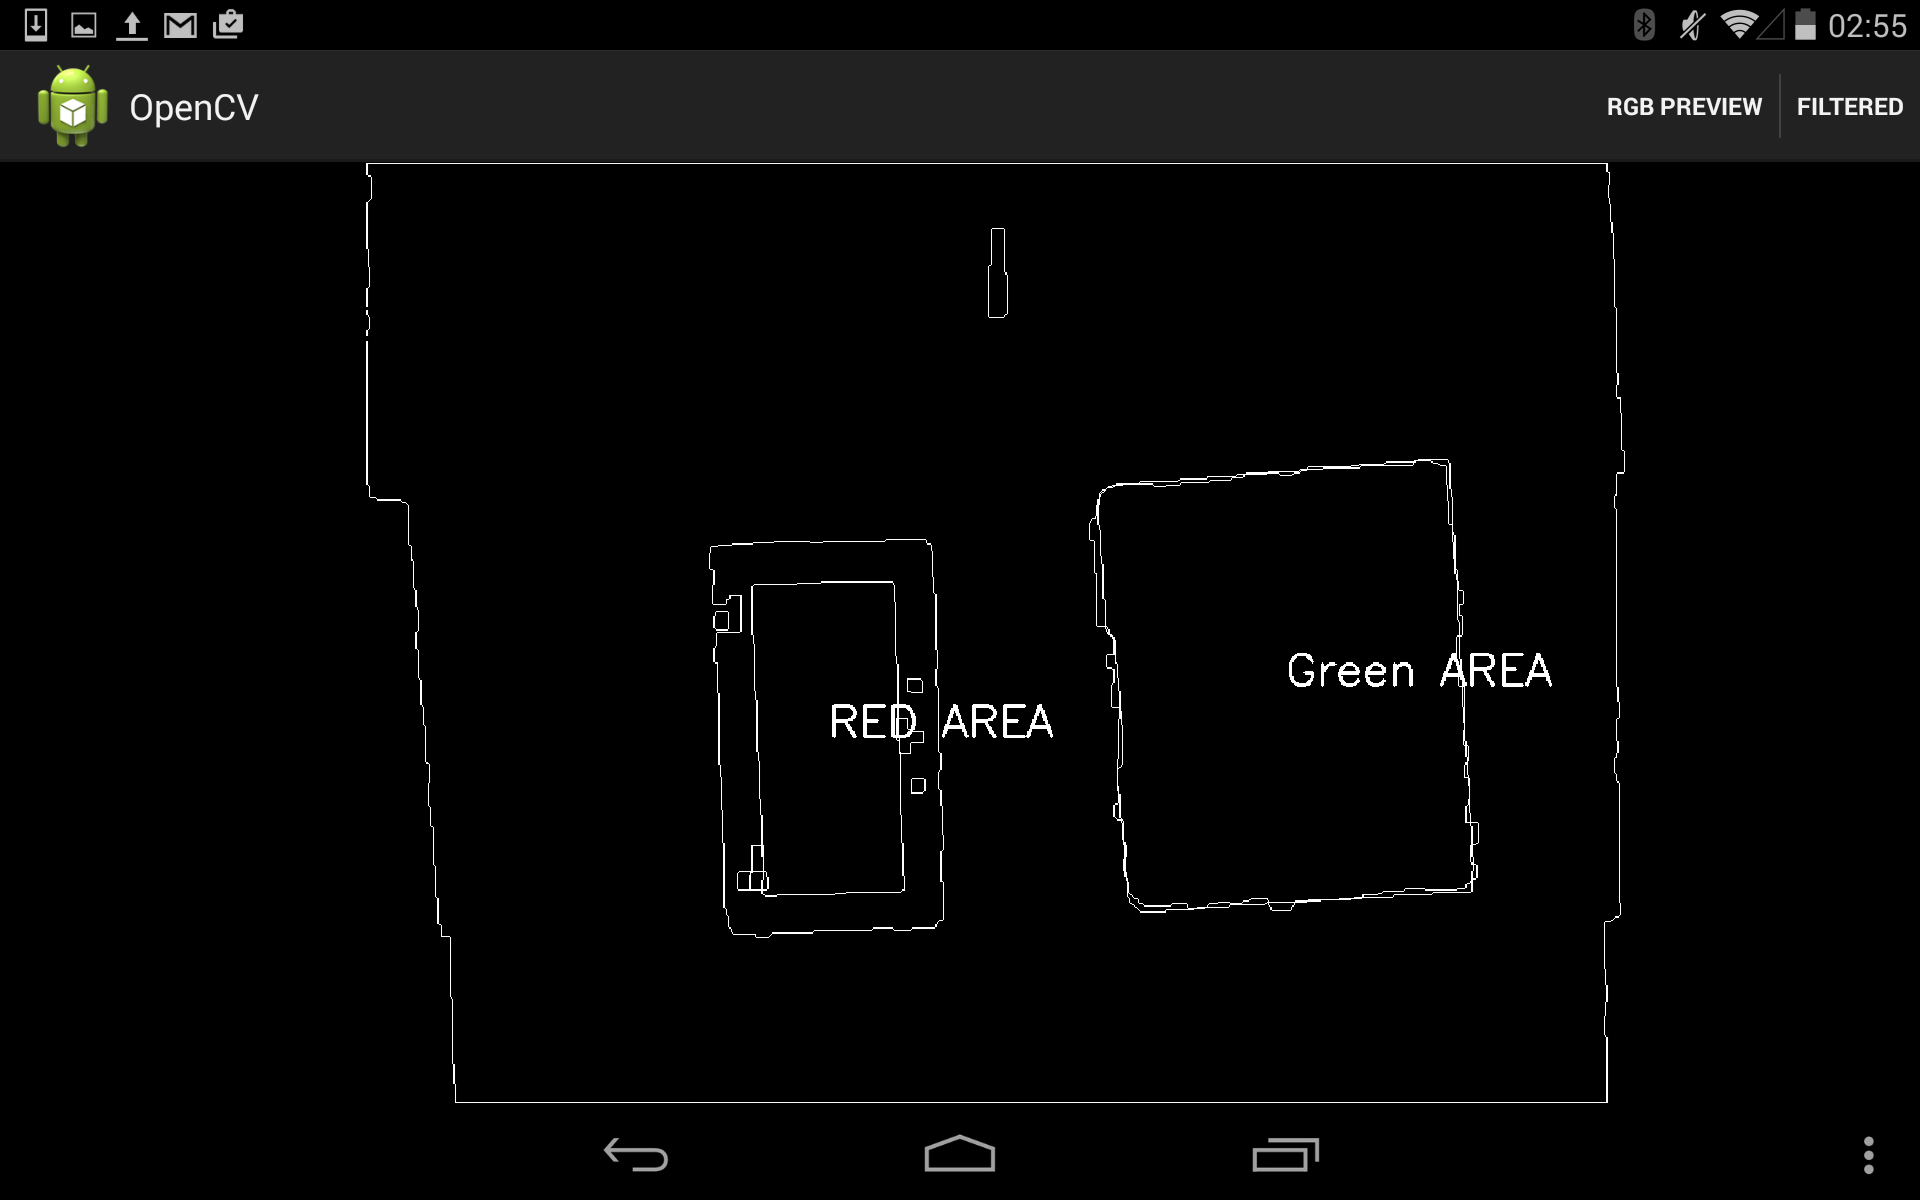
\includegraphics[width=\textwidth]{multiple(filtered)}
        \caption{Same frame filtered for Multiple colours}
    \end{subfigure}
    \hfill
    \caption{Screenshot of the application working for Multiple colour area}
     \label{filtered_multiple}
\end{figure}



\subsubsection{TableApp} \label{tableapp}

The second half of the application is the TableApp. This is the app that should show the relevant content  of the interactive table and also handle the interactions. It should also help to keep track of number of devices on the table.

Whenever this application starts a new session, by hitting the \emph{submit button} of the session screen, shown in Figure \ref{session_screen}, it queries the data store for number of devices in the session and updates the value. This number is also used to determine the colour identification of this device and subsequently flash this colour to identify its initial position. Figure \ref{red_screen} shows the outcome of having the screen filled with a colour.As well as updating the, number of devices, field of the database it initialises its own position to (0,0) and waits for the CameraApp to update its position before removing the background colour. If it is the first device then it initialises the number of devices to be 1 and sets zoom to be 1 as well.

When the device is detected by the CameraApp, it updates the position in the data store. The advantage of Firebase is that when the value gets changed if you have a listener for it, it gets called automatically simulating a push notification. When the device receives the notification it removes the colour overlay and shows the image at that position.

One of the drawbacks of using Firebase as the data store was the lack of support for real numbers. Firebase only has support for Long and Integers types which meant that it was quite difficult to store zoom values properly. The compromise we decided to make was to convert the zoom value into a String and save it as a String and then convert it back to a Double value when the application requires it.


